% pierwsza sekcja
\section{Wprowadzenie}

Nowe technologie oraz wzrost popularności urządzeń mobilnych (ang. \emph{smartphone}) otwierają nowy obszar działań w dziedzinie marketingu, a w szczególności kreowania i wzmacniania marki w świadomości konsumentów. Odpowiednio przygotowany marketing wirusowy (ang. 
\emph{viral marketing}) poprzez rozpowszechnianie informacji przez samych potencjalnych klientów, może przyczynić się do dużego zasięgu informacji na temat marki (na przykład w mediach społecznościowych) zerowym kosztem dalszej propagacji informacji. Działania te mogą bezpośrednio wpłynąć na wysoką konwersję sprzedaży w kontekście dostarczenia informacji konsumentowi końcowemu od znajomego, z polecenia, co buduje większe zaufanie. W połączeniu z coraz bardziej popularną techniką angażowania konsumenta - grywalizacją (inaczej grywalizacją, ang. \emph{gamification}) w sposób dla niego przyjemny, wspomaga budowanie wizerunku marki.

Ostatecznym efektem działań w ramach pracy dyplomowej jest stworzenie prototypu technologii, która może być wykorzystana jako gra marketingowa wyświetlana na ekranie LED umieszczonym w centrum miasta lub w klubie, sterowana bezpośrednio ze smartfona bez konieczności instalacji jakiejkolwiek aplikacji dedykowanej na dany system operacyjny, aby zminimalizować próg wejścia do gry do niezbędnego minimum (np. do wpisania adresu w przeglądarkę internetową lub zeskanowania QR Code [ang. \emph{Quick Response Code}]).

Możemy wyobrazić sobie sytuację, że na mieście pojawia się ekran LED, na którym przechodnie mogą wysterować grą miejską angażującą klientów danej marki w postaci zdobycia punktów z możliwością ich wymiany lub osiągnięciem statusu ambasadora marki. Informacja rozchodzi się po sieci w mediach społecznościowych w postaci nagrań filmów, natomiast firma inicjująca formę grywalizacji bezkosztowo propaguje informacje utwierdzające jej istnienie wśród konsumentów.

Korzystając z faktu powstania technologii WebSocket protocol (ustandaryzowanej przez IETF\footnote{Internet Engineering Task Force} w 2011 roku w dokumencie RFC\footnote{Request for Comments} 6455\cite{websockets-rfc}) umożliwiającą dwukierunkową transmisję danych pomiędzy przeglądarką internetową oraz serwerem poprzez gniazdo (ang. \emph{socket})  wspieraną przez większość przeglądarek zainstalowanych na urządzeniach mobilnych. Intencją pracy dyplomowej jest stworzenie mechanizmu sterowania komputerem z poziomu przeglądarki internetowej uruchomionej na urządzeniu mobilnym bez konieczności instalacji zewnętrznego oprogramowania w postaci aplikacji dedykowanej dla danego systemu operacyjnego. Korzystając również z faktu, iż aktywni użytkownicy urządzeń mobilnych chętnie aktualizują oprogramowanie, wprowadzenie tej technologii zwiększa zasięg użytkowników, którzy mogą skorzystać z technologii z każdą aktualizacją (200 milionów uaktualnionych urządzeń firmy Apple\footnote{Statystyki z oficjalnych press release firmy Apple, uaktualnienie systemu operacyjnego do iOS7 http://www.apple.com/pr/library/2013/09/23First-Weekend-iPhone-Sales-Top-Nine-Million-Sets-New-Record.html} oraz pokrycia ponad 55,6 proc. Androida w wersji 4.1 i powyżej \footnote{Statystyki z dnia 02.12.2013 r. http://developer.android.com/about/dashboards/index.html}).

Realizacja pracy dyplomowej uwzględnia również optymalizację rozmiaru oraz sposobu ładowania kodu do przeglądarki internetowej na urządzeniu mobilnym mając na uwadze dostęp do wolniejszej sieci 3G (niż w przypadku dostępu do szerokopasmowej sieci Internet lub LTE [ang. \emph{Long Term Evolution}, nazywany inaczej 4G LTE]). W celu szybszego ponownego (przy kolejnych odwiedzinach) ładowania statycznej treści wykorzystany został \emph{Local Sotorage}\cite{webstorage} wprowadzony wraz z HTML5, ustandaryzowany przez W3C\footnote{World Wide Web Consortium} w dokumencie W3C Recommendation Web Storage, a do serwowania statycznej treści po raz pierwszy został zbudowany lokalny CDN (ang. \emph{Content Delivery Network}) złożony z Varnish Cache.

\begin{figure}[h!]
  \caption{A picture of a gull.}
  \centering
    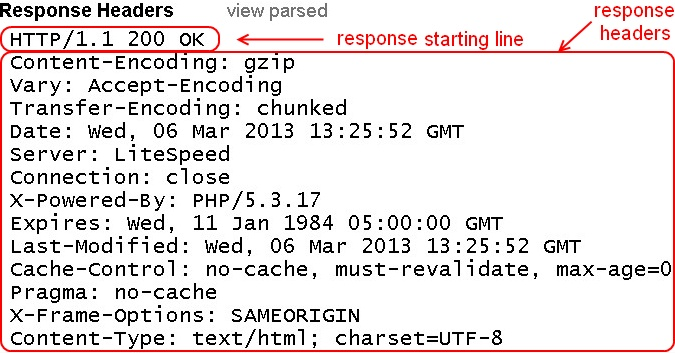
\includegraphics{testimage}
\end{figure}
